\subsection{Główna struktura interfejsu}

Przygotowano interfejs zgodnie z ustalonymi wymaganiami. W celu ułatwienia pracy w wielu edytorach w
tym samym czasie, zaimplementowano system zakładek. Zaimplementowano możliwość przełączania motywu
aplikacji z jasnego na ciemny i odwrotnie. Główny interfejs zamieszczono na rysunku
\ref{mainInterfaceFigure}.

\begin{figure}
    \centering
    \subfloat[\centering Motyw jasny]
        {{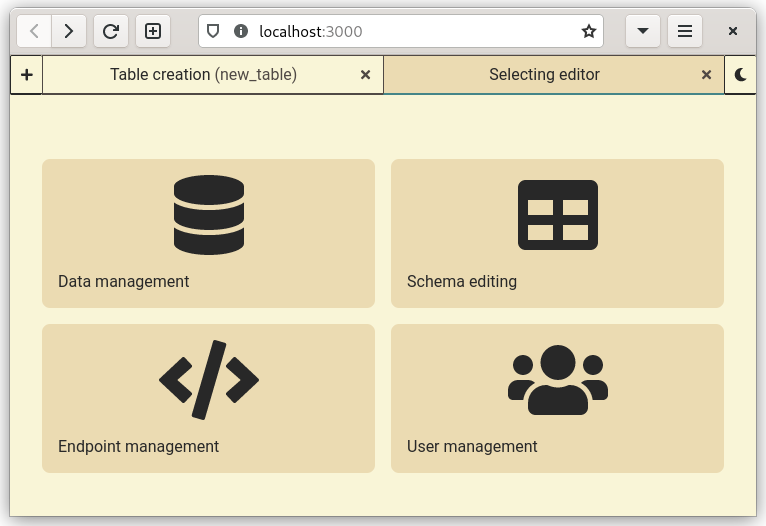
\includegraphics[width=.45\linewidth]{./img/starting_view_light.png} }}
    \qquad
    \subfloat[\centering Motyw ciemny]
        {{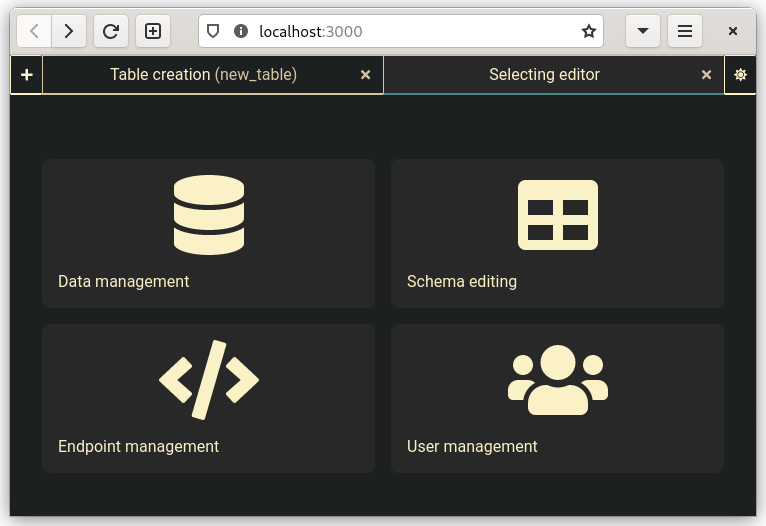
\includegraphics[width=.45\linewidth]{./img/starting_view_dark.png} }}

    \caption{Główny interfejs aplikacji}
    \label{mainInterfaceFigure}
\end{figure}

